% !TeX spellcheck = de_DE
\documentclass{alex_gp}

\name{Alexander Helbok}
\course{Grundpraktikum}
\hwnumber{1}


\begin{document}

\begin{myfigure}{Datenaufzeichnung}{12}
	\begin{wrapfigure}{r}{0.5\textwidth}
			\vspace{-1em}
			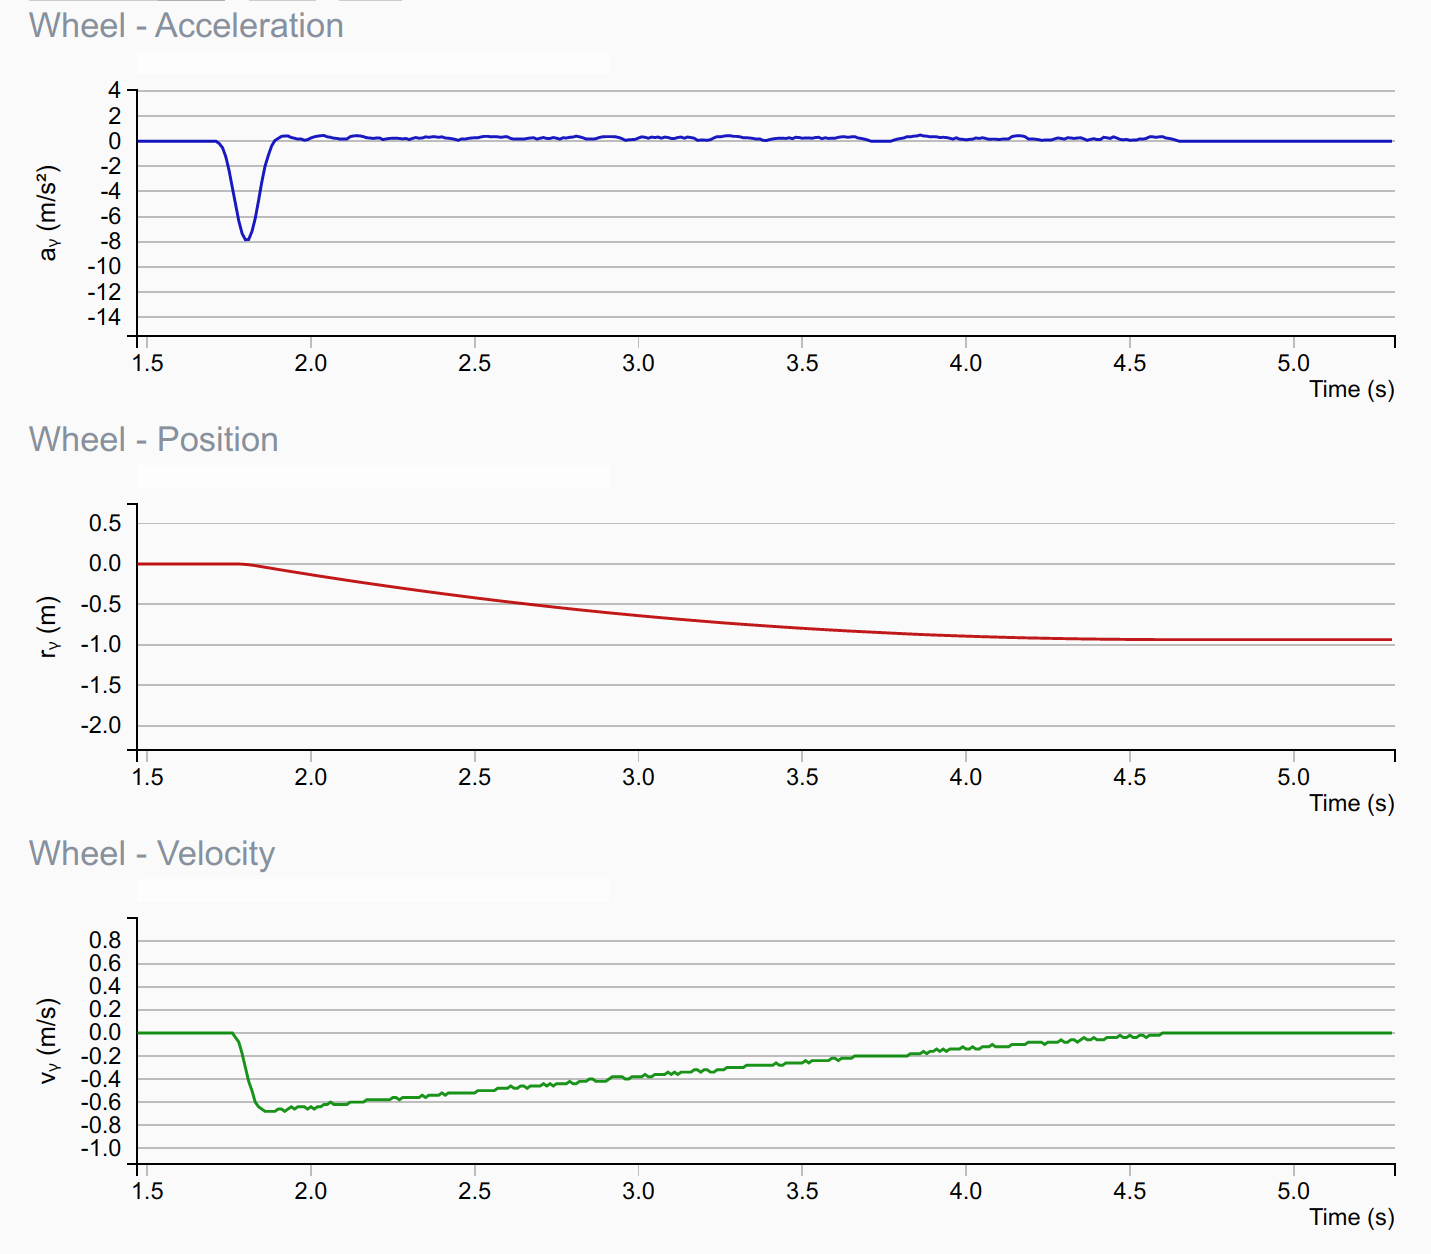
\includegraphics[width=0.5\textwidth]{Versuch1 - 2}
			\caption{Von oben nach unten sind Beschleunigung, Ort und Geschwindigkeit des Messgeräts auf die Zeit aufgetragen. Nur der relevante Zeitabschnitt wird dargestellt.}
	\end{wrapfigure}
	In der nebenstehenden Abbildung sieht man jeweils die Beschleunigung, die Geschwindigkeit und den Ort des IOLab Messgeräts auf die Zeit aufgetragen. 
	Der oberste Plot zeigt die Beschleunigung in Bewegungsrichtung, in Rot sieht man die Position in Bezug auf die Anfangslage, und der grüne Graph stellt die Geschwindigkeit des Geräts dar. \par
	
	\indent Das Gerät befindet sich anfänglich in Ruhe bis der Stoß kommt, was sich im Beschleunigungs- und Geschwindigkeitsgraphen als starker negativer Anstieg erkenntlich macht. 
	Nach dem Stoß geht die Beschleunigung zu etwas über 0 zurück und die Geschwindigkeit des Geräts verringert konstant (aufgrund von Reibung). Der Ortsgraph flacht mit der Zeit ab, da das IOLab Gerät immer langsamer wird und somit weniger Weg in der gleichen Zeit zurücklegt. \par
	
	Zum Schluss steht das Gerät still und die Graphen nehmen eine konstante ein.
\end{myfigure}
\begin{mybox}{Analysewerkzeuge}
	\begin{tabular}{@{}r rrr c rrr c rrr@{}}\toprule
		& \multicolumn{3}{c}{Intervall 1} & \phantom{ac}& \multicolumn{3}{c}{Intervall 2} &	\phantom{ac} & \multicolumn{3}{c}{Intervall 3}\\
		\cmidrule{2-4} \cmidrule{6-8} \cmidrule{10-12}
		& $\vec{x}\quad$ & $\vec{v}\quad$ & $\vec{a}\quad$ && $\vec{x}\quad$ & $\vec{v}\quad$ & $\vec{a}\quad$ && $\vec{x}\quad$ & $\vec{v}\quad$ & $\vec{a}\quad$\\ \midrule
		$\mu$ & -0.479 & -0.475 & 0.270 && -0.684 & -0.347 & 0.250 && -0.825 & -0.222 & 0.211\\
		$\sigma$ & 0.036 & 0.022 & 0.071&& 0.026 & 0.020 & 0.090 && 0.017 & 0.020 & 0.12\\
		$s$ & -0.47 & 0.26& -0.52&& -0.34& 0.23& -0.44&& -0.22& 0.25& -1.00\\
		$\Delta$ & -0.118 & 0.080& 0.037&& -0.087& 0.060& 0.090&& -0.055& 0.060& -0.230\\
		$a$ & -0.120 & -0.119& 0.067&& -0.171& -0.087& 0.063&& -0.206& -0.055& 0.053\\
		\bottomrule
	\end{tabular}
	\captionof{table}{Mittelwert, Standardabweichung, Steigung der angepassten Gerade, Veränderung im Funktionswert und Zeitintegral für jeweils Ort, Geschwindigkeit und Beschleunigung in drei verschiedenen Intervallen}
	\label{table:1}
	\tcbbreak
%	\begin{minipage}[0.4\textheight]{\textwidth}
%		\begin{multicols}{2}
%			\centering
%			\begin{tabular}{c| c || c  c  c} 
%			\hline
%				\multicolumn{2}{c ||}{} & \( \mu \) & \( \sigma \) & s \\ [0.5ex] 
%			\hline\hline
%				\multirow{3}{*}{\rotatebox{90}{Intervall 1}} & 
%				\( \vec{x} \) & -0.479 & 0.036 & -0.47 \\ 
%				& \( \vec{v} \) & -0.475 & 0.022 & 0.26 \\
%				& \( \vec{a} \) & 0.270 & 0.071 & -0.52 \\ [1ex] 
%			\hline
%				\multirow{3}{*}{\rotatebox{90}{Intervall 2}} & 
%				\( \vec{x} \) & -0.684 & 0.026 & -0.34 \\ 
%				& \( \vec{v} \) & -0.347 & 0.020 & 0.23 \\
%				& \( \vec{a} \) & 0.250 & 0.090 & -0.44 \\ [1ex] 
%			\hline
%				\multirow{3}{*}{\rotatebox{90}{Intervall 3}} & 
%				\( \vec{x} \) & -0.825 & 0.017 & -0.22 \\ 
%				& \( \vec{v} \) & -0.222 & 0.020 & 0.25 \\
%				& \( \vec{a} \) & 0.211 & 0.12 & -1.00 \\ [1ex] 
%			\hline
%			\end{tabular}
%			\captionof{table}{Mittelwert, Standardabweichung und Steigung der angepassten Gerade für jeweils Ort, Geschwindigkeit und Beschleunigung in drei verschiedenen Intervallen}
%		\columnbreak
%			\begin{figure}[H]
%				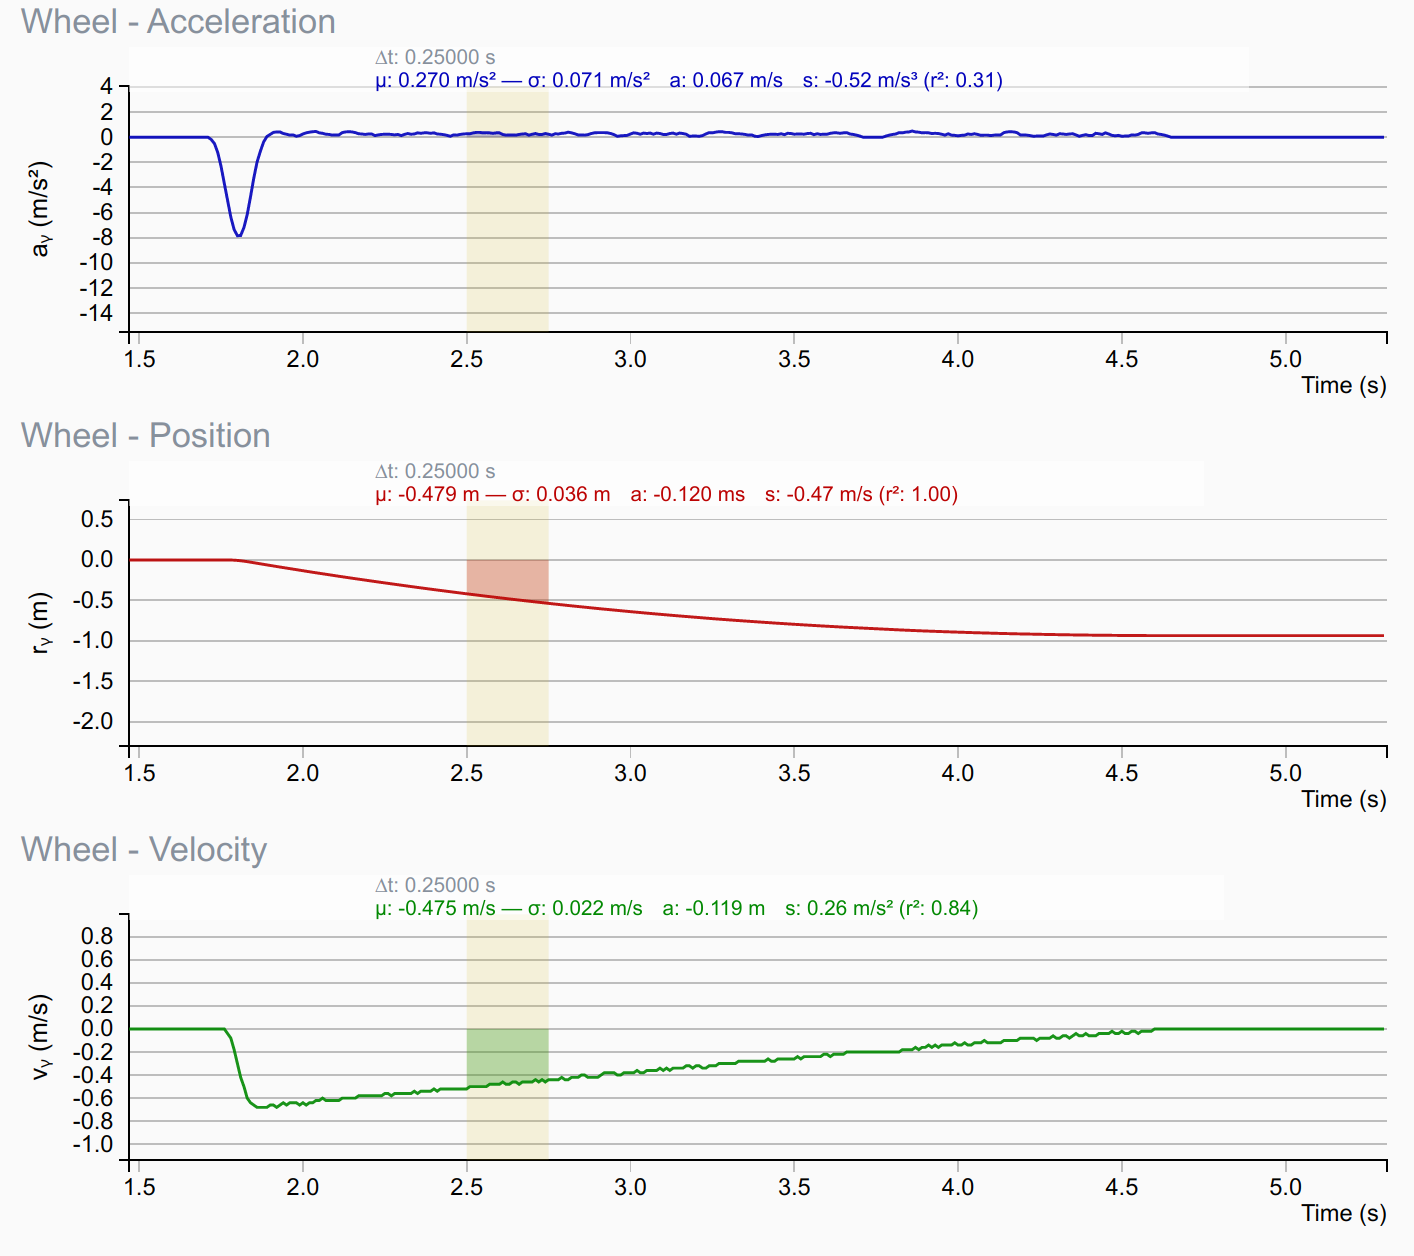
\includegraphics[width=0.5\textwidth]{Versuch1 - 3}
%				\caption{Von oben nach unten sind Beschleunigung, Ort und Geschwindigkeit des Messgeräts auf die Zeit aufgetragen. Statische Daten beziehen sich auf das Intervall 1}
%			\end{figure}
%		\end{multicols}
%	\vspace{1em}
%	\end{minipage}
%		\tcbbreak
		\noindent Es wurden 3 Intervalle ab \( t = 2.5 \unit{s}, 3 \unit{s}, 3.5 \unit{s} \) und Länge \( \Delta t = 0.25 \unit{s} \) gewählt und jeweils der Mittelwert \( \mu \), die Standardabweichung \( \sigma \) und die Steigung \( s \) einer angepassten Gerade berechnet. Diese Gleichungen
		\begin{equation}
			\label{eqn:diff}
			\vec{v} = \dv{\vec{x}}{t};\quad \vec{a} = \dv{\vec{v}}{t}
		\end{equation}
		stellen einen Zusammenhang zwischen Ort, Geschwindigkeit und Beschleunigung her. In unserem Fall werden \( \vec{v}, \vec{a} \) als Mittelwert \( \mu \) berechnet und \( \dv{\vec{x}}{t}, \dv{\vec{v}}{t} \) werden durch eine Tangente mit Steigung \( s \) approximiert. Daher stimmen die Werte auch nicht ganz überein, weil eine Gerade das Verhalten nicht exakt beschreibt (wie die r Werte auch zeigen). Dennoch stellen die Daten keinen Widerspruch dar, weil die berechnete Steigung weit innerhalb des \( 1\sigma \) Intervalls des Mittelwerts liegt.\par
		
		Gleichung \ref{eqn:diff} kann man auch zu
		\begin{equation}
			\label{eqn:int}
			\vec{x} - \vec{x}_0 = \uint[t_0, t]{\vec{v}}{t};\quad \vec{v} - \vec{v}_0 = \uint[t_0, t]{\vec{a}}{t} 
		\end{equation}
		umschreiben, um so die Differenz im Funktioniert \( \Delta \) auf das Zeitintegral \( a \) der Ableitung zurückzuführen. Dies ist auch in Tabelle \ref{table:1} zu sehen, wobei die Werte wieder nicht exakt übereinstimmen, weil das Integral numerisch approximiert wird (eine analytische Lösung hier nicht möglich ist). \par
		\begin{figure}[H]
			\centering
			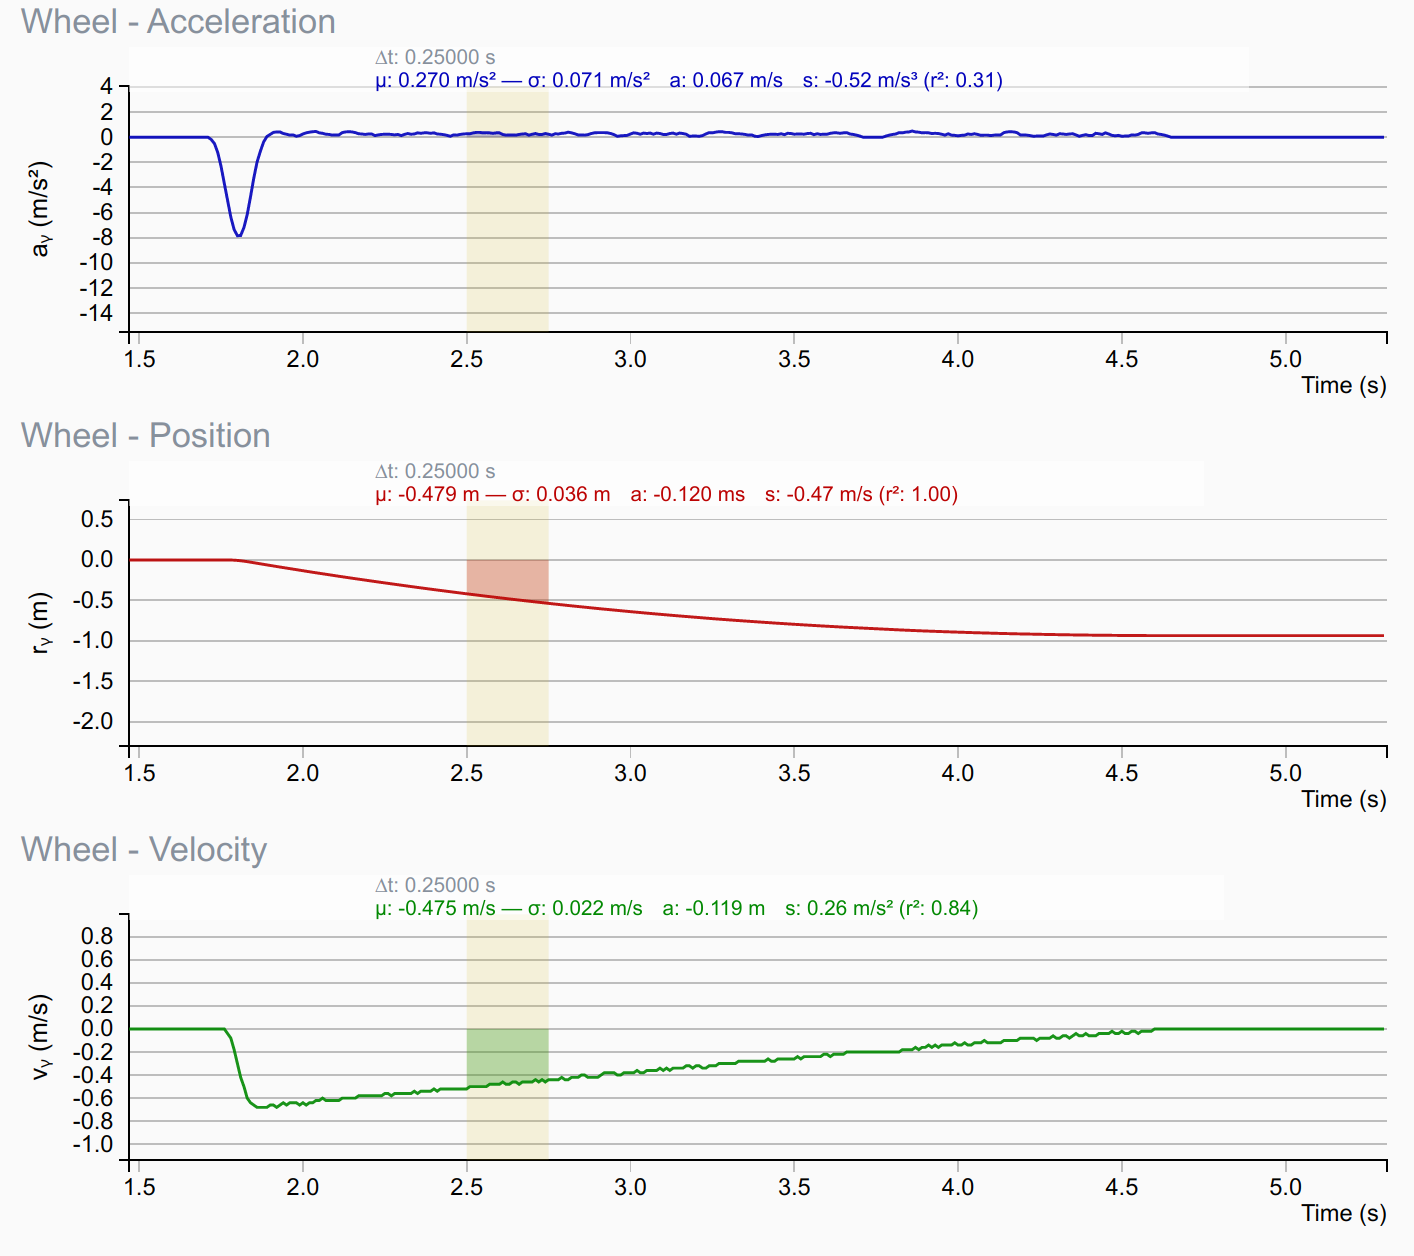
\includegraphics[width=0.75\textwidth]{Versuch1 - 3}
			\caption{Von oben nach unten sind Beschleunigung, Ort und Geschwindigkeit des Messgeräts auf die Zeit aufgetragen. Statische Daten beziehen sich auf das Intervall 1}
		\end{figure}
\end{mybox}
\newpage
\begin{mybox}{Analyse}
	\begin{figure}[H]
		\vspace{-0.5cm}		
		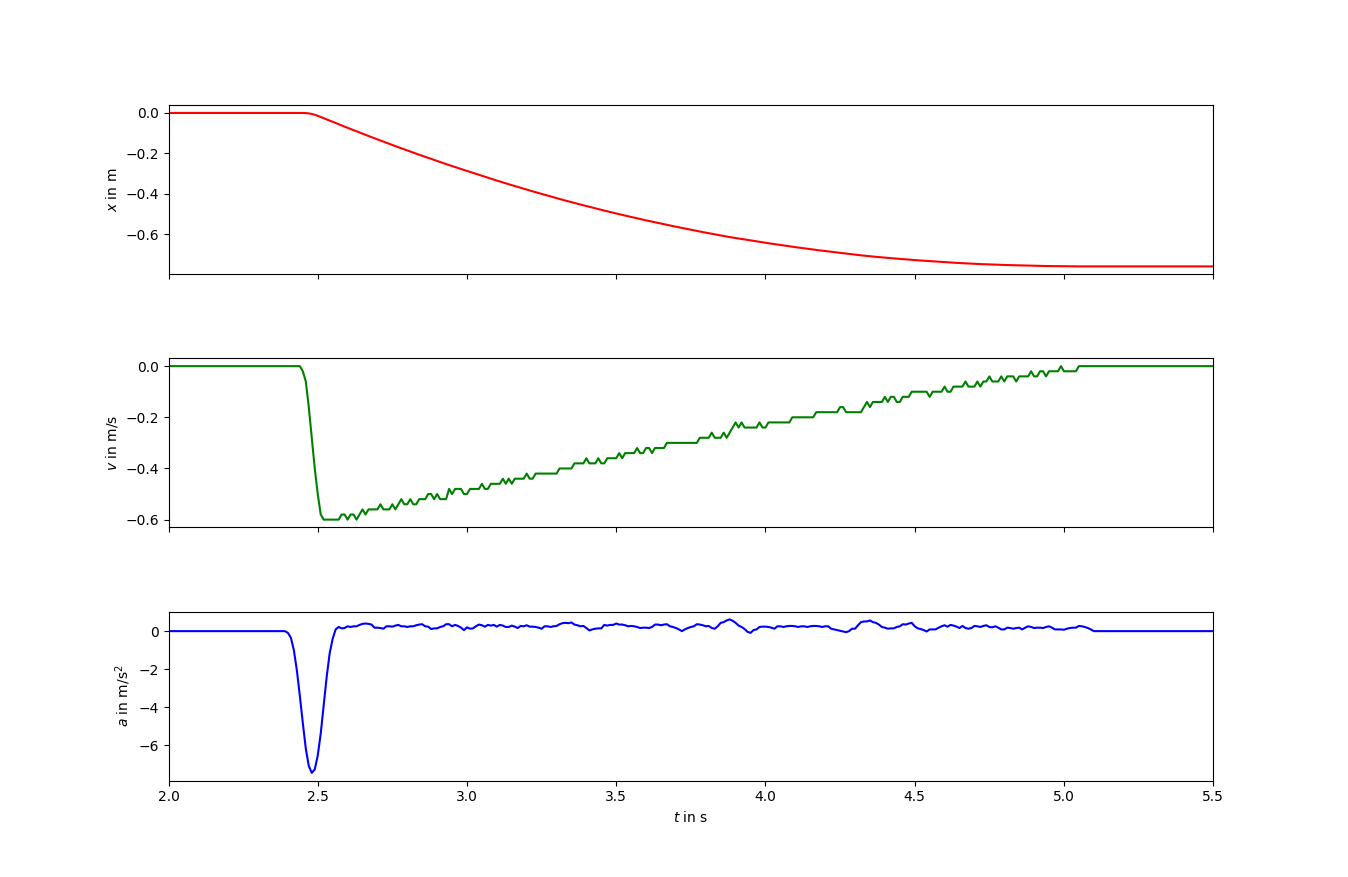
\includegraphics[width=\textwidth]{Versuch1 - 1}
		\caption{Von oben nach unten sind Ort, Geschwindigkeit und Beschleunigung des Messgeräts auf die Zeit aufgetragen. Nur der relevante Zeitabschnitt wird dargestellt.}
	\end{figure}
\end{mybox}

\end{document}